\subsubsection{\stid{6.01} LANL ATDM Software Technologies}

%%%%%%%%%%%%%%%%%%%%%%%%%%%%%%%%%%%%%%%%%%%%%%%%%%%%%%%%%%%%%%%%%%%%%
\paragraph{Overview} \leavevmode \\

The LANL ATDM PMR effort is focusing on the development and use of
advanced programming models for Advanced Technology Development and
Mitigation (ATDM) use-cases. Our current focus is on research and development
of new programming model capabilities in the \textbf{Legion} data-centric
programming system. Legion provides unique capabilities that align
well with our focus on the development of tools and technologies that
enables a separation of concerns of computational physicists and
computer scientists. Within the ATDM PMR effort we have focused on the
development of significant new capabilities within the Legion runtime
that are specifically required to support LANL's ATDM
applications. Another key component of our work is the co-design and
integration of advanced programming model research and development
within \textbf{FleCSI}, a Flexible Computational Science Infrastructure. A
major benefit to the broader ECP community is the development of new 
features in the Legion programming system which are available as free
open-source software \url{https://gitlab.com/StanfordLegion/legion}.  

The \textbf{Kitsune} Project, part of LANL's ATDM CSE efforts, provides a
compiler-focused infrastructure for improving various aspects of the
exascale programming environment.  At present, our efforts are primarily
focused on advanced LLVM compiler and tool infrastructure to support the
use of a \emph{parallel-aware} intermediate representation.  In
addition, we are actively involved in the Flang Fortran compiler that
is now an official sub-project within the overall LLVM infrastructure.
All these efforts include interactions across ECP as well as
with the broader LLVM community and industry.  

The LANL ATDM Data and Visualization project develops scalable
solutions for data analysis as part of the \textbf{Cinema} project,
which provides post-facto interactive interactions with a dataset
using a fraction of the file storage. 

The \textbf{BEE/Charliecloud} subproject is creating software tools to increase portability
and reproducibility of scientific applications on high performance and cloud
computing platforms.  Charliecloud \cite{priedhorskyrrandlestc2016} is an unprivileged Linux container
runtime.  It allows developers to use the industry-standard Docker
\cite{dockerinc}
toolchain to containerize scientific applications and then execute them on
unmodified DOE facility computing resources without paying any performance
penalty.  BEE \cite{beeproject} (Build and Execution Environment) is a toolkit providing
users with the ability to execute application workflows across a diverse set of
hardware and runtime environments.  Using Bee's tools, users can build and
launch applications on HPC clusters and public and private clouds, in
containers or in containers inside of virtual machines, using a variety of
container runtimes such as Charliecloud and Docker. 



%%%%%%%%%%%%%%%%%%%%%%%%%%%%%%%%%%%%%%%%%%%%%%%%%%%%%%%%%%%%%%%%%%%%%
\paragraph{Key  Challenges} \leavevmode \\

\subparagraph{Legion:}

Applications will face significant challenges in realizing sustained performance on next-generation systems. Increasing system complexity coupled with increasing scale will require significant changes to our current programming model approaches. This is of particular importance for large-scale multi-physics applications where the application itself is often highly dynamic and can exhibit high variability in resource utilization and system bottlenecks depending on what physics are currently in use (or emphasized). Our goal in the LANL ATDM PMR project is to support these highly dynamic applications on Exascale systems, providing improvements in productivity, long-term maintainability, and performance portability of our next-generation applications. 

\subparagraph{FleCSI Legion integration:}
FleCSI is a Flexible Computational Science Infrastructure whose goal is to provide a common framework for application development for LANL's next-generation codes. FleCSI is required to support a variety of different distributed data structures and computation on these data structures including structured and unstructured mesh as well as mesh-free methods. Our work in the LANL ATDM PMR project is focused on co-designing the FleCSI data and execution model with the Legion programming model to ensure the latest advancements in the programming model and runtimes research community are represented in our computational infrastructure. A significant challenge in our work is the additional constraint that FleCSI must also support other runtime systems such as MPI. Given this constraint, we have chosen an approach that ensures functional correctness across both runtimes but that also leverages and benefits from capabilities in Legion that are not directly supported in MPI (such as task-based parallelism as a first-class construct). 

\subparagraph{Kitsune:}
A key challenge to our efforts is reaching agreement within the broader community that
a parallel intermediate representation is beneficial and needed within
LLVM.  This not only requires showing the benefits but also providing a
full implementation for evaluation and feedback from the community.
In addition, significant new compiler capabilities represent a
considerable effort to implement and involve many complexities and technical
challenges.  These efforts and the process of up-streaming potential
design and implementation changes do involve some amount of time and
associated risk. 

Additional challenges come from a range of complex issues surrounding
target architectures for exascale systems.  Our use of the LLVM
infrastructure helps reduce many challenges here since many processor
vendors and system providers now leverage and use LLVM for their
commercial compilers.

\subparagraph{Cinema}
Interfacing to a large number of ECP application with the Cinema
software and the management of the volumous data from these
applications. 

\subparagraph{Bee/CharlieCloud}
Other HPC-focused container runtimes exist, such as NERSC's Shifter
\cite{canonrsjacobsend} and
Singularity \cite{kurtzergmsochatvbauermw}.  These alternative runtimes have characteristics, such as
complex setup requirements and privileged user actions, that are undesirable in
many environments.  Nevertheless, they represent a sizable fraction of the
existing HPC container runtime mindshare.  A key challenge for BEE is
maintaining support for multiple runtimes and the various options that they require
for execution.  This is especially true in the case of Singularity, which
evolves rapidly.  Similarly, there is a diverse collection of resources that
BEE and Charliecloud must support to serve the ECP audience.  From multiple HPC
hardware architectures and HPC accelerators such as GPUs and FPGAs, to
differing HPC runtime environments and resource managers, to a multitude of
public and private cloud providers, there is a large set of available resources
that BEE and Charliecloud must take into consideration to provide a
comprehensive solution.

%%%%%%%%%%%%%%%%%%%%%%%%%%%%%%%%%%%%%%%%%%%%%%%%%%%%%%%%%%%%%%%%%%%%%
\paragraph{Solution Strategy} \leavevmode \\

\subparagraph{Legion:}

In funded collaboration with NVIDIA, LANL and NVIDIA are developing new features in Legion to support our applications. Necessary features are identified through direct engagement with application developers and through rapid development, evaluation, and refactoring within the team. Major features include Dynamic Control Replication for improved scalability and productivity and Dynamic Tracing to reduce runtime overheads for  applications with semi-regular data dependencies such as applications with stencil-based communication patterns. 


\subparagraph{FleCSI Legion integration:}
LANL staff work on co-design and integration of the Legion programming system into the FleCSI framework. We have regular milestones that align well with application needs and the development of new features within Legion. 


\begin{figure}[htb]
  \centering
  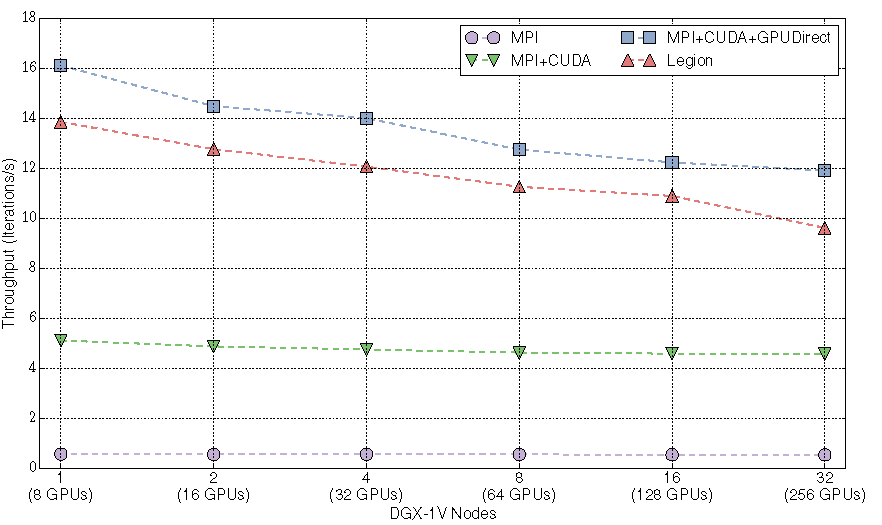
\includegraphics[width=4in]{projects/2.3.6-NNSA/2.3.6.01-LANL-ATDM/control-replication-performance}
        \caption{\label{fig:control-replication-performance}\textbf{Productivity features such as Dynamic Control Replication scales well across multi-GPU systems in unstructured mesh computations.}}
\end{figure}

\begin{figure}[htb]
        \centering
        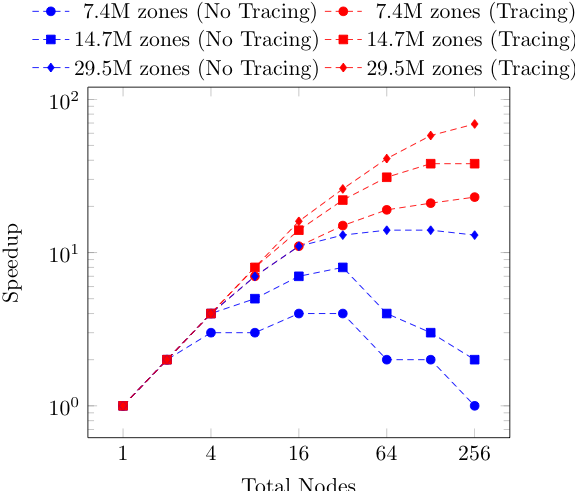
\includegraphics[width=4in]{projects/2.3.6-NNSA/2.3.6.01-LANL-ATDM/tracing-performance}
        \caption{\label{fig:tracing-performance}\textbf{New Legion features such as Tracing will improve strong scaling in unstructured mesh computations.}}
\end{figure}


\subparagraph{Kitsune:}
Given the project challenges, our approach takes aspects of
today's node-level programming systems (e.g. OpenMP and Kokkos) and
popular programming languages (e.g. C++ and Fortran) into
consideration and aims to improve and expand upon their capabilities
to address the needs of ECP.  This allows us to attempt to strike a
balance between incremental improvements to existing infrastructure
and more aggressive techniques that seek to provide innovative
solutions, thereby managing risk while also providing the ability to introduce new
breakthrough technologies.

Unlike current designs, our approach introduces the notion of explicit
parallel constructs into the LLVM intermediate representation, building
off of work done at MIT on Tapir~\cite{2.3.6.01:kitsune:Schardl:2017}. 
We are exploring extensions to this work as well as making some changes
to fundamental data structures within the LLVM infrastructure to assist with
and improve analysis and optimization passes. 


\subparagraph{Cinema:}
The LANL Cinema project is focused on delivering new
visualization capabilities for creating, analyzing, and managing data for
Exascale scientific applications and Exascale data centers.

Cinema~\cite{cinema:Ahrens:SC14} is being developed in coordination with
LANL's ECP application NGC to ensure that data collected during the simulation
execution is of appropriate frequency, resolution, and viewport for later
analysis and visualization by scientists. Cinema is an innovative way of
capturing, storing and exploring extreme scale scientific data. Cinema is
essential for ECP because it embodies approaches to maximize insight from
extreme-scale simulation results while minimizing data footprint 

\subparagraph{Bee/CharlieCloud:}
The BEE/Charliecloud project is focusing first on providing support for
containerized production LANL scientific applications across all of the
existing LANL production HPC systems.  The BEE/Charliecloud components required
for production use at LANL will be documented, released and fully supported.
Follow-on development will focus on expanding support to additional DOE
platforms.  This will mean supporting multiple hardware architectures,
operating systems, resource managers, and storage subsystems.  Support for
alternative container runtimes, such as Docker, Shifter, and Singularity is
planned.

%%%%%%%%%%%%%%%%%%%%%%%%%%%%%%%%%%%%%%%%%%%%%%%%%%%%%%%%%%%%%%%%%%%%%
\paragraph{Recent Progress} \leavevmode \\

\subparagraph{Legion:} 
One of the strengths of Legion is that it executes asynchronous tasks as if they were executed in the sequence they occur in the program. This provides the programmer with a mental model of the computation that is easy to reason about. However, the top-level task in this tree-of-tasks model can often become a sequential bottleneck, as it is responsible for the initial distribution of many subtasks across large machines. In earlier work NVIDIA developed the initial implementation of control replication, which allows the programmer to write tasks with sequential semantics that can be  transparently replicated many times, as directed by the Legion mapper interface, and run in a scalable manner across many nodes.
Dynamic control replication is an important capability for LANL's ATDM effort, allowing our application teams to write applications with apparently sequential semantics while enabling scalability to Exascale architectures. This approach will improve understandability of application code, productivity, and composability of software and ease the burden of optimization and porting to new architectures. 
New dynamic tracing ability has been added to Legion to allow debugging and insight in to peformance optimization activites.

\subparagraph{FleCSI Legion Integration:} 
A key component of LANL's Advanced Technology  Development and Mitigation effort is the development of a flexible computational science infrastructure (FleCSI) to support a breadth of application use cases for our Next Generation Code. FleCSI has been co-designed with the Legion programing system in order to enable our Next Generation Code to be performance portable and scalable to future Exascale systems. Legion provides the underlying distributed and node-level runtime environment required for FleCSI to leverage task and data parallelism, data dependent execution, and runtime analysis of task dependencies to expose parallelism. We completed testing of Legion on Sierra with a Visco-Plastic Self-Consistent, VSCP, application to investigate initial performance on GPU systesm.

\subparagraph{Kitsune:}
Our primary focus is the delivery of capabilities for LANL's ATDM
Ristra application (AD 2.2.5.01).  In support of the requirements for
Ristra, we are targeting the lowering of Kokkos constructs directly
into the parallel-IR representation.  At present, this requires
explicit lowering of Kokkos constructs and we have basic support
for \texttt{parallel\_for} and \texttt{parallel\_reduce} in place.  In
addition we are looking at replacement of LLVM's dominator tree, a key
data structure for optimizations including parallelization and
memory usage analysis, with a \emph{dominator directed-acyclic-graph}
(DAG).  This work is currently underway and should near its initial
implementation early in the 2020 calendar year.  In addition, we are
actively watching recent events within the LLVM community around
multi-level intermediate representations (MLIR) and the relationship
they have with parallel semantics, analysis, optimization, and code
generation.  Furthermore, we are participating in ongoing discussions within the
community about general details behind parallel intermediate forms. 



\subparagraph{Cinema:}

Recent Cinema work has focused on development of analysis capability, Exascale workflows and working with ECP STs such as ALPINE to enable in situ and post processing production of Cinema databases.  Currently Cinema is available in situ via ParaView Catalyst and Ascent and available post hoc via ParaView and VisIt.   New capabilities provide scientists more options in analyzing and exploring the results of large simulations by providing a workflow that 1) detects features in situ, 2) captures data artifacts in Cinema databases, 3) promotes post-hoc analysis of the data, and 4) provides data viewers that allow interactive, structured exploration of the resulting artifacts. 
%
In our most recent milestone, we ran two end-to-end simulation pipelines with ECP applications at scale to generate Cinema databases and ran Cinema-based workflows with Cinema algorithms to produce secondary set of artifacts.  We ran (1) Nyx integrated with Ascent, running the ALPINE adaptive sampling algorithm; and (2) SW4 integrated with Ascent, running a VTK-m isocontour algorithm.  

\subparagraph{Bee/CharlieCloud}
% previous recent progress
%Recent Charliecloud progress has been focusing on understanding and documenting
%best practices for running large scale MPI jobs using containerized runtimes.
%Additional work has been done to enhance support for using containers with
%GPUs.  Charliecloud is available at https://github.com/hpc/charliecloud and was
%recently approved for inclusion in the next release of OpenHPC.
%
%BEE currently has beta-level support for launching Charliecloud containers on
%LANL HPC systems.  Automated BEE scalability testing is nearing production
%readiness.
Recent Charliecloud progress has focused on understanding and documenting best
practices for running large scale MPI jobs using containerized runtimes.
Charliecloud is enhancing support for multiple MPI implementations.
Charliecloud is available at https://github.com/hpc/charliecloud and is
distributed inside of Debian and Gentoo Linux distributions as well as being
part of OpenHPC.  Charliecloud won an 2018 R\&D-100 award.

BEE fully supports launching Charliecloud containers on all LANL HPC systems.
It can also launch containers on AWS and OpenStack clouds such as NSF
Chameleon.  BEE also supports interactive launching of jobs with the SLURM
resource manager. BEE was shown at the end of FY19 to support a complex multiphysics application with setup, in situp visualization and checkpoint-restart on a production system at LANL.

%%%%%%%%%%%%%%%%%%%%%%%%%%%%%%%%%%%%%%%%%%%%%%%%%%%%%%%%%%%%%%%%%%%%%
\paragraph{Next Steps} \leavevmode \\

\subparagraph{Legion:} 
Focus on hardening and scalability of Legion's Dynamic Control Replication and development of Dynamic Tracing for application use-cases. 

\subparagraph{FleCSI Legion Integration:} 
Support the Ristra Application milestone to run on Sierra and Trinity.

\subparagraph{Kitsune:}
The key next step for our feature set is to complete implementation of Kokkos use cases 
that match the needs of Ristra.  Where possible, we will also
explore the broader set of use cases within ECP's overall use of
Kokkos constructs.  The Kitsune toolchain is still very much an
active \emph{proof-of-concept} effort based on Clang (C and C++) with
plans to add support for Fortran via the newly established Flang front
end within LLVM (ST 2.3.2.12).  Even though it is not yet production
ready, we are actively updating and releasing source code and the supporting
infrastructure for deployment as an early evaluation candidate.  In
addition to these components, we will actively begin to explore targeting
the exascale systems (Aurora, Frontier, and El Capitan).


\subparagraph{Cinema:}
Cinema is focusing on outreach to ECP applications to identify new application workflows that can be reasonably made efficient and working on new analysis methods for Cinema users.

\begin{figure}[htb]
	\centering
	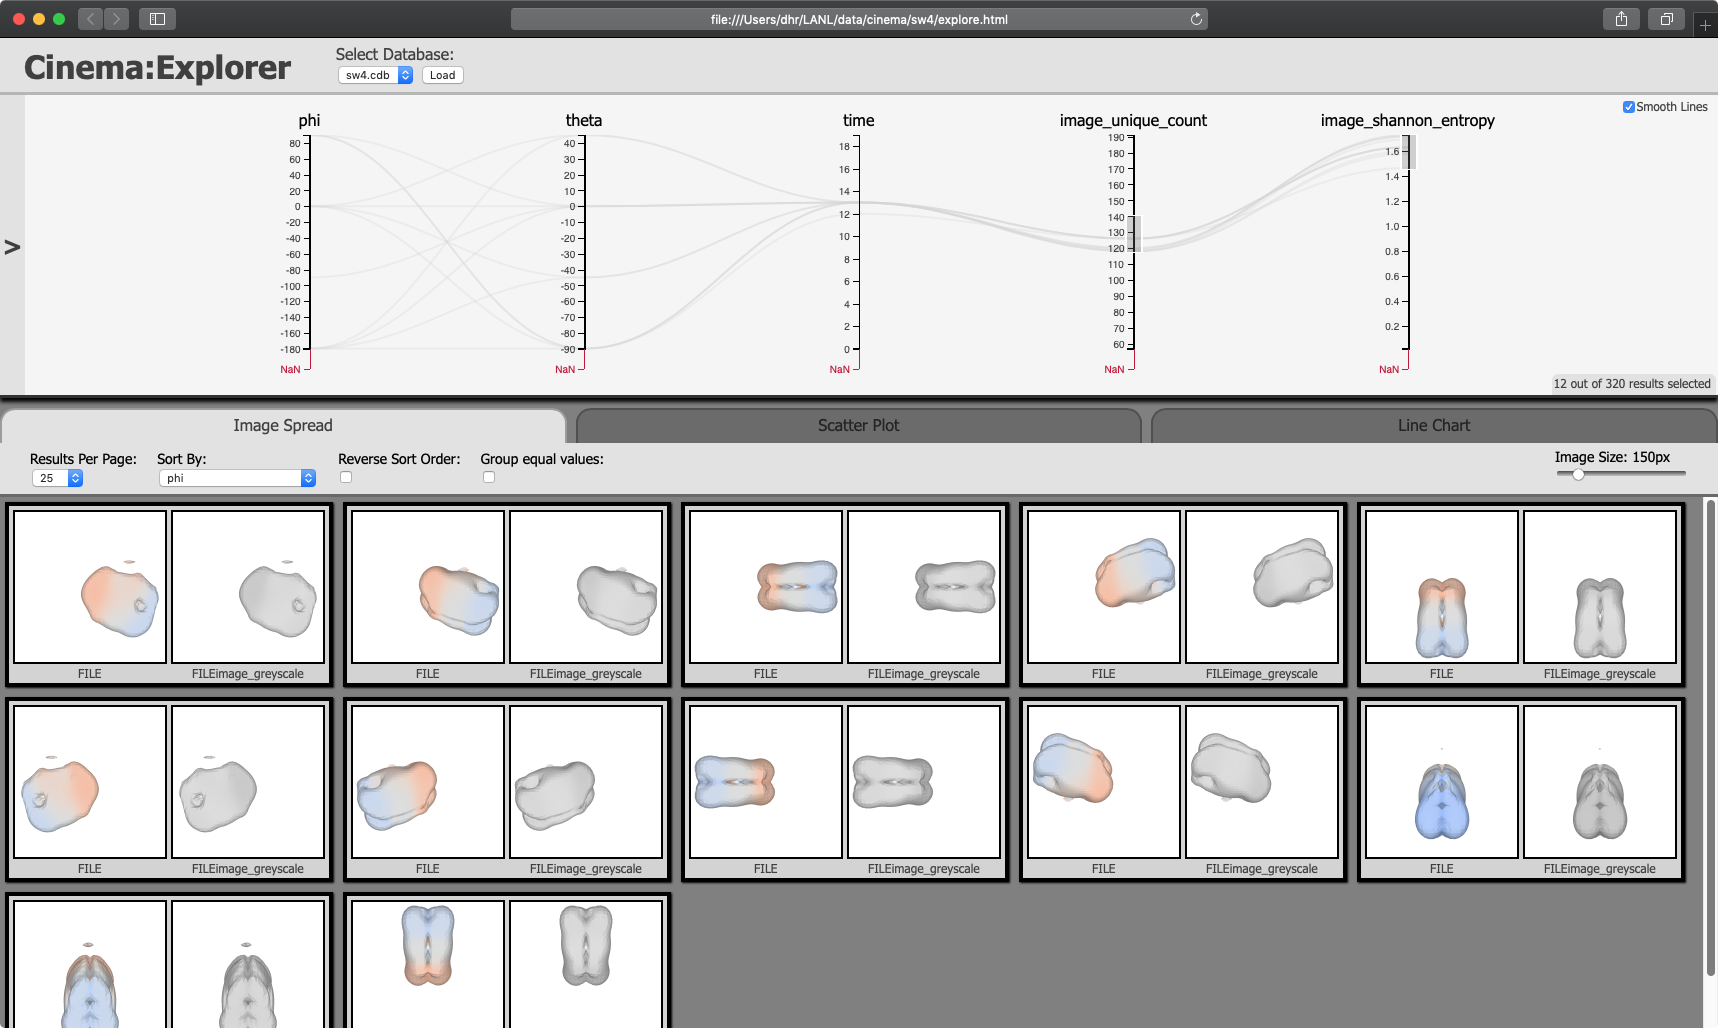
\includegraphics[width=4in]{projects/2.3.6-NNSA/2.3.6.01-LANL-ATDM/cinema-sw4-example.png}
	\caption{
		Screen capture of a browser-based viewer displaying the results of a analysis workflow using an SW4 isocontour Cinema database.  
	\label{fig:cinema-sw4example}
	}
\end{figure}

\subparagraph{Bee/CharlieCloud}
A refactoring of BEE to support an open standard is underway. Support for the Open Workflow standard will allow a base on a well defined workflow description language leveraged by other scientiic communities. This will then be tested on multiple systems to ensure portability.
